\documentclass{article}
\usepackage{url,amsmath}
\usepackage{epsfig,caption}

\newcommand{\SnAPhyl}{SNAPP}

\title{A rough guide to \SnAPhyl}
\author{Remco Bouckaert, David Bryant\\
\url{remco@cs.auckland.ac.nz, david.bryant@otago.ac.nz}\\
Auckland University\\
}

\begin{document}
\maketitle

\section{Introduction}

\SnAPhyl\ is a program to perform MCMC analysis on SNP and AFLP data using the
method described in \cite{SnAPhyl}. It is released under the lesser GPL licence.
Source code is available on request to the authors.
Executables for Mac, Linux and Windows are available for download from
\url{http://snapp.otago.ac.nz/}.


\section{Typical usage}

In summary:
\begin{itemize}
\item Prepare input file, setting data, priors, initial tree and mcmc operators and options.
See Section \ref{sec.prep} for details on settings and Section \ref{sec.beauti} for details
on how to use Beauti to set up an analysis file for \SnAPhyl.
\item Run \SnAPhyl\ (see Section \ref{sec.cmd} for details).
\item Analyze the trace, e.g. using {\tt Tracer}\footnote{Part of BEAST, or separately available 
from \url{http://beast.bio.ed.ac.uk/Tracer}} (see Section \ref{sec.trace} for details), 
and depending on whether the chain converged, rerun with longer chain or other parameters.
\item Analyze tree file by using the TreeSetAnalyser and DensiTree programs packaged with SNAPP,
or alternatively using {\tt splitstree}\footnote{Available from \url{http://www.splitstree.org/}},
 {\tt figtree}\footnote{Available from \url{http://tree.bio.ed.ac.uk/software/figtree/}}
(see Section \ref{sec.tree} for details).
\end{itemize}

\newpage

\section{Preliminaries: variables and parameters}

\SnAPhyl\ is an MCMC program that takes AFLP (or SNP) data and produces a sample from the posterior distribution of species trees (and their parameters). There are four kinds of variable in the sample:
\begin{itemize}
\item The species tree topology;
\item The branch lengths in the species tree, or equivalently, the divergence times for nodes in the species tree;
\item The forward and backward mutation rates;
\item The effective population size for each ancestral population in the species tree, given in terms of $\theta$.
\end{itemize}
A real source of confusion, both for \SnAPhyl\ and similar methods, is that the rates of mutation and times are confounded, so we typically rescale the units of time. To make this explicit, here are some of the standard population parameters and their units:\\

\begin{tabular}{rlp{2.5in}}
\hline 
$\mu$ & mutation rate & expected number of mutations per site per generation \\
$g$ & generation time& length of generation time, in years \\
$N$ & effective population size & number of individuals  \\ 
$\theta$ & average divergence & expected number of mutations between two individuals \\ \hline \\
\end{tabular}
For a diploid population, $\theta = 4N\mu$. If $\mu$ is instead the expected number of mutations per site per year then we would have $\theta = 4N \mu g$. 

In the analysis in \cite{SnAPhyl} we measured time in terms of expected number of mutations. Hence
\begin{itemize}
\item The expected number of mutations per unit time is $1$;
\item A branch of length $\tau$ in the species tree corresponds to $\tau / \mu$ generations, or $\tau g / \mu$ years.
\item The backward and forward mutation rates, $u$ and $v$, were constrained so that the total expected number of mutations per unit time is 1, which gives
\[ \frac{v}{u+v} u + \frac{u}{u+v} v = 1.\]
\item The $\theta$ values are unaffected by this rescaling. If the true mutation rate $\mu$ is known, then the $\theta$ values returned by the program can be converted into effective population sizes using 
\[N = \theta/(4 \mu).\]
\end{itemize}


\section{Preparing input file\label{sec.prep}}
\SnAPhyl\ uses an XML file as its specification. The easiest ways to create this XML file are to (i) use Beauti to create an XML file
as outlined in Section \ref{sec.beauti}, or (ii) export an appropriately formatted snaphyl file from SplitsTree.

To prepare the input file, the following items need to be specified: SNP or AFLP data,
prior parameters, starting tree and MCMC parameters, as explained below.



\if0
\subsection{Data}
The data used by \SnAPhyl\ is the summary data per species; for every species, we need
the number of lineages and for SNP data the number of lineages in a species with a
particular number of SNPs present (the number of 'reds' per site).

\subsection{Priors}

\SnAPhyl\ uses a {\em Yule prior} for the species tree and branch lengths on the species tree. This prior has a single parameter, $\lambda$, which governs the rate that species diverge. This rate, in turn, determines the (prior) expected height of the species tree, which we denote by $r$. The formula connecting these is two quantities is
\[\lambda = \frac{1}{r}  \left(\sum_{k=1}^{n-1} \frac{k}{n(n-k)}\right)\]
where $n$ is the number of species , which can be used to specify the $\lambda$ value giving the desired root height.


The theta ($\theta$) values for the ancestral population sizes all have gamma distribution priors. The parameters for the gamma distributions are the same over the entire tree, and for all trees, and the prior distribution for each ancestral population are independent. There are two parameters determining the gamma distribution:
\begin{itemize}
\item the shape parameter $\alpha$;
\item the scale parameter $\beta$.
\end{itemize}
Note that the mean of the prior distribution if $\alpha/\beta$ while the variance of the prior distribution is $\alpha/(\beta)^2$.

At present, the MCMC does not sample values for the backwards and forward mutation rates, $u$ and $v$. These are fixed at their initial values. We note that, given these rates, the stationary frequencies of the two states are $\pi_0 = v/(u+v)$ and $\pi_1 = u/(u+v)$, while the mutation rate is 
\[\pi_0 u + \pi_1 v = \frac{2uv}{u+v}.\]
Hence, given an estimate for $\pi_0$, and the constraint that the mutation rate is $1$, we can solve for $u$ and $v$ as
\begin{eqnarray*}
u & = & \frac{1}{2\pi_0} \\
v & = & \frac{1}{2\pi_1} \\
& = & \frac{1}{2(1-\pi_0)}.
\end{eqnarray*}

%

%A justifiable estimate for $\lambda$ can be obtained as follows. First, estimate the
%height of the tree, which is determined by the largest distance between two lineages 
%in the data. If this distance is $d$ then $r=d/2$ is the estimate of the tree height.
%Let $n$ be the number of species, then 
%$$\lambda=\frac{1}{n\cdot r}\sum_{k=1}^{n-1}\frac{k}{n-k}.$$

%The values for $\alpha$ and $\beta$ are the parameters for a gamma distribution (???)
%and can be estimated from the data as follows;
%for every species $S$, calculate the expected distance $d(x,y)$ among lineages
%$$\sum_{x,y\in S}\frac{d(x,y)}{\binom{|S|}{2}}$$ 
%This is the sum over
%all pairs of lineages for a species of the fraction $d(x,y)$ of SNPs where the two lineages
%differ, divided by the number of pairs (i.e., $\binom{|S|}{2}=|S|(|S|-1)/2$ for a species with $|S|$ lineages).
%For the set of species, calculate mean $m$ and variance $\sigma$, then $\beta=m/\sigma$
%and $\alpha = m*\beta$ are good estimates. To make the prior more conservative,
%divide $\alpha$ and $\beta$ by $10$.


\subsection{Starting values}

There are three ways to choose a starting tree for the chain:
\begin{enumerate}
\item create a UPGMA tree using  Nei genetic distance,
\item read a starting tree in Newick format; or 
\item generate a random tree from the prior distribution (recommended).
\end{enumerate}
The $\theta$ values on this tree will be drawn from the prior gamma distributions.

\subsection{MCMC parameters}

The MCMC parameters include the
length of the chain, 
the interval at which the chain is logged, 
the items to be logged,
and the specifics of the operators (proposals) and their parameters.

\newpage
\fi

\subsection{Using Beauti\label{sec.beauti}}

After starting Beauti, the first thing to do to specify an analysis is importing an alignment of
SNP or AFLP data. Select the File/Import alignment menu item and a file chooser pops up with
which the file containing an alignment in Nexus format can be selected. If an analysis file was
saved before, it can be loaded back into Beauti by using the File/Load menu.


\begin{minipage}{\textwidth}
\captionof{figure}{\label{fig.beauti1}Importing an alignment in Beauti}
\begin{center}
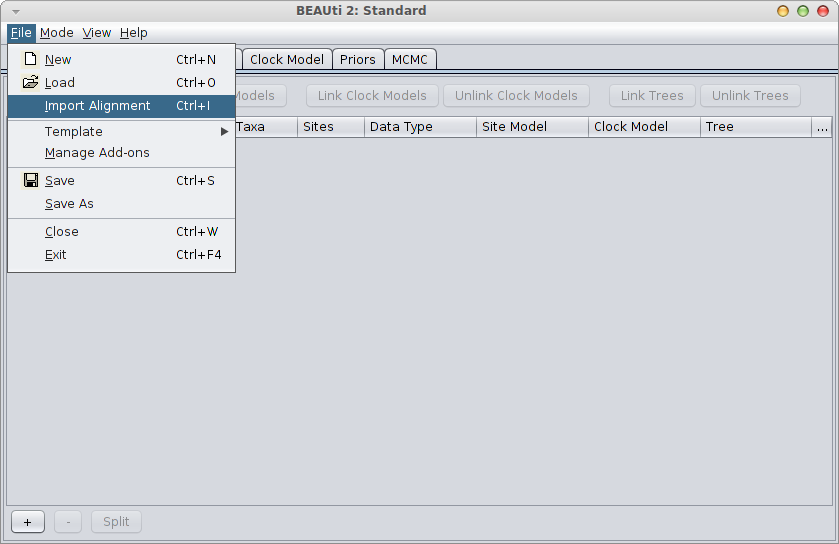
\includegraphics[width=0.8\textwidth]{figures/Beauti-import.png}
\end{center}
\end{minipage}

\subsubsection{Beauti taxon set editing}

When loading an alignment, Beauti guesses which of the alignments form a species by looking at
the separator characters ('.','-','\_' and ',') in taxon names. However, you should carefully
go through the taxon sets and make corrections if necessary. Taxon sets can be renamed by editing 
the labels in the tree. Taxa can be moved around using drag an drop. To highlight taxa names
matching part of a name, the filter entry at the top of the tree can be used. All taxon 
names matching\footnote{A regular expression of the form ".*[filter entry text].*" is used for matching.}
the text in the filter are highlighted, the remainder greyed out. 

\begin{minipage}{\textwidth}
\captionof{figure}{\label{fig.beauti2}Editing taxon sets in Beauti}
\begin{center}
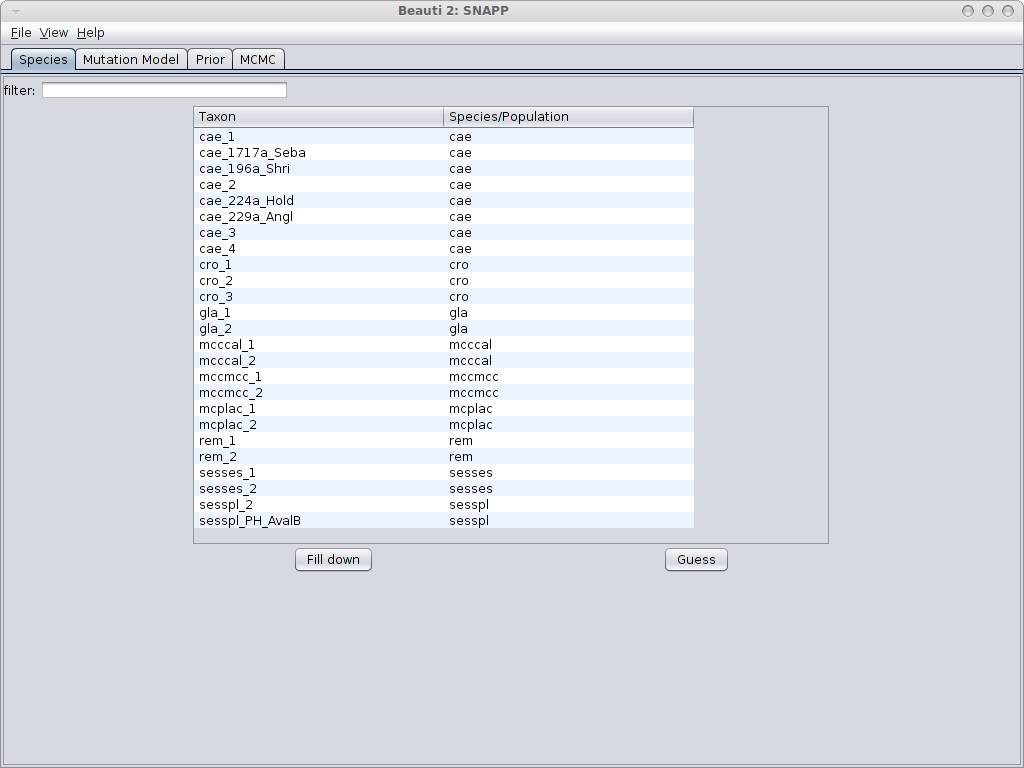
\includegraphics[width=0.75\textwidth]{figures/Beauti-taxonsets.png}
\end{center}
\end{minipage}


\subsubsection{Beauti mutation model settings}

Click the tab 'mutation model' to show u, v and coalescent rate parameters and a number 
of optional check boxes.
By default, the MCMC does not sample values for the backwards and forward mutation rates,
$u$ and $v$. These are fixed at their initial values. We note that, given these rates, 
the stationary frequencies of the two states are $\pi_0 = v/(u+v)$ and $\pi_1 = u/(u+v)$, 
while the mutation rate is \[\pi_0 u + \pi_1 v = \frac{2uv}{u+v}.\]
Hence, given an estimate for $\pi_0$, and the constraint that the mutation rate is $1$, we can solve for $u$ and $v$ as
\begin{eqnarray*}
u & = & \frac{1}{2\pi_0} \\
v & = & \frac{1}{2\pi_1} \\
& = & \frac{1}{2(1-\pi_0)}.
\end{eqnarray*}

A fixed value can be entered, which will be used as initial value. When clicking
the 'sample' check box, the parameter will be estimated during the course of the
MCMC chain. Click the little button with the 'e' on the right to specify
bounds on a parameter that is sampled.
When sampling a parameter a prior on the parameter need to be specified (which
will show up automatically under the 'prior' tab).



\begin{minipage}{\textwidth}
\captionof{figure}{\label{fig.beauti3}Mutation model parameters in Beauti}
\begin{center}
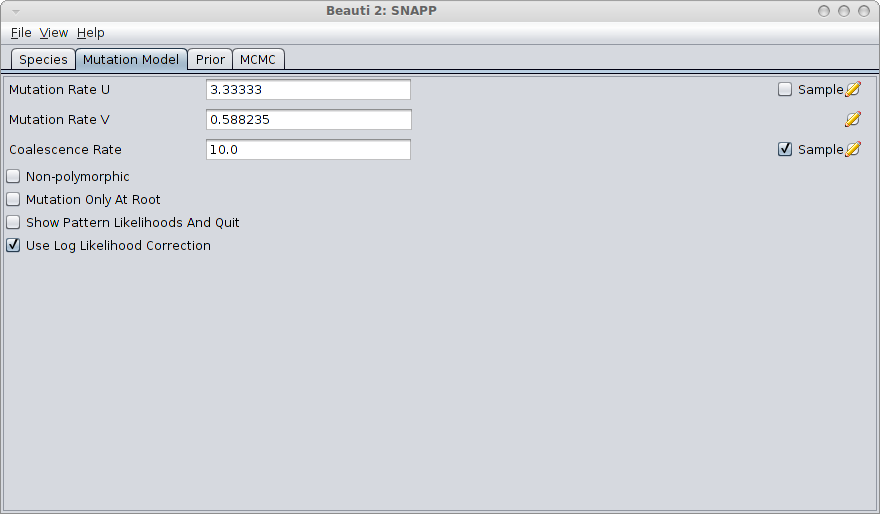
\includegraphics[width=0.75\textwidth]{figures/Beauti-model.png}
\end{center}
\end{minipage}

The ``non-polymorphic'' checkbox signals to SNAPP that only
polymorphic (variable) sites have been included in the data
(all constant sites are ignored). It is important to check this box if
SNP data is being used, as the likelihood
calculations are quite different if SNAPP assumes all constant sites
have already been removed.

The "mutationOnlyAtRoot" checkbox indicates conditioning on zero mutations, except 
at root (default false).
As a result, all gene trees will coalesce in the root only, and never in any of the branches.

It is possible to indicate whether alleles are dominant, however in our experience this
only leads to much longer run times without changing the analysis significantly. Therefore
it is set to false by default.

\subsubsection{Beauti tree prior settings}

Click the 'prior' tab to show the prior used in the analysis. 
\SnAPhyl\ uses a {\em Yule prior} for the species tree and branch lengths on the species tree. This prior has a single parameter, $\lambda$, which governs the rate that species diverge. This rate, in turn, determines the (prior) expected height of the species tree, which we denote by $r$. The formula connecting these is two quantities is
\[\lambda = \frac{1}{r}  \left(\sum_{k=1}^{n-1} \frac{k}{n(n-k)}\right)\]
where $n$ is the number of species, which can be used to specify the $\lambda$ value giving the desired root height.

\subsubsection{Beauti rate prior settings}

The theta ($\theta$) values for the ancestral population sizes all have gamma distribution priors by default. 
This can be altered by selecting the combobox and selecting one of 'gamma', 'inverse gamma', 'CIR' or 'uniform'.
The parameters for the gamma distributions are the same over the entire tree, and for all trees, and the prior distribution for each ancestral population are independent. There are two parameters determining the gamma distribution:
\begin{itemize}
\item the shape parameter $\alpha$;
\item the scale parameter $\beta$.
\end{itemize}
Note that the mean of the prior distribution if $\alpha/\beta$ while the variance of the prior distribution is $\alpha/(\beta)^2$.

\begin{minipage}{\textwidth}
\captionof{figure}{\label{fig.beauti4}Prior settings in Beauti}
\begin{center}
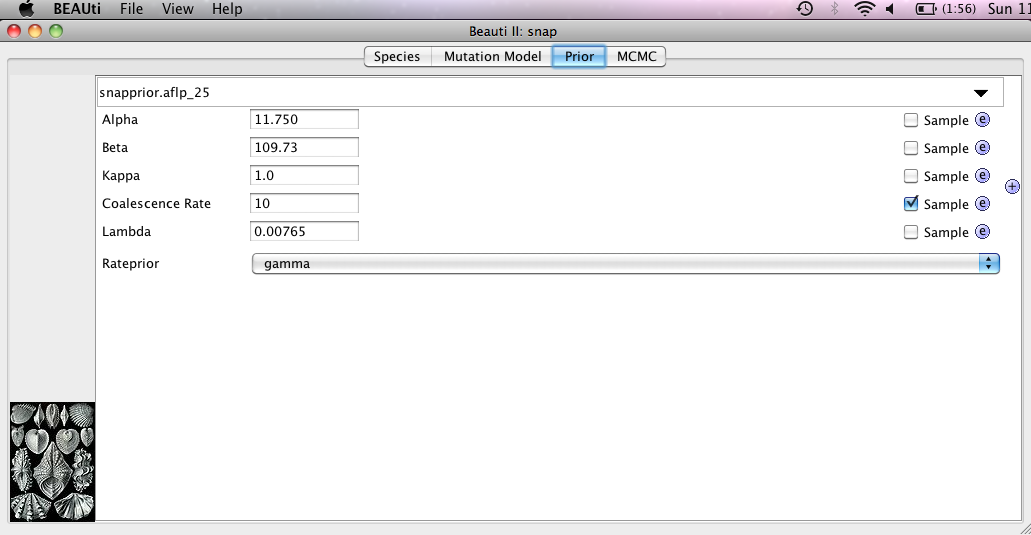
\includegraphics[width=0.75\textwidth]{figures/Beauti-prior.png}
\end{center}
\end{minipage}

When selecting 'inverse Gamma' we assume independent inverse gamma distributions for thetas,
so $(2/r)$ has an inverse gamma (alpha,beta) distribution. That means that $r$ has density proportional to
 $1/(r^2) * INVGAMMA(2/r|alpha,beta)$.

When selecting the CIR process \cite{CIR}, the kappa parameter is used as well.
			 The CIR process has SDE
			 $$dr = \kappa (\theta - r) dt + \sigma \sqrt{r} dz_1$$
			 has a stationary distribution that is gamma with 
				$$\alpha = 2 \kappa \theta / \sigma^2$$
			 and 
				$$\beta = 2 \kappa / \sigma^2$$
			 The correlation between time 0 and time $t$ is  $exp(-\kappa t)$.
			 
			 
			 Let $c = 2 \kappa / (\sigma^2 * (1 - exp(-\kappa t)))$
			 
			 If we condition on rate $r0$ at time 0, the distribution of $2*c*rt$ is non-central
			 chi squared with 
				$$2q+2 = 4\kappa \theta / \sigma^2$$  
			 degrees of freedom and parameter of non-centrality
				$$2u = c r_0 exp(-\kappa t)$$
			 
			 
			 Converting these into our set of parameters (alpha, beta, kappa) we have
			 $$\theta = \alpha / \beta$$
			 $$\sigma^2 = 2 \kappa / \beta$$
			 so
			 $$c = \beta/(1 - exp(-\kappa t))$$
			 $$df = 2q+2 = 2 \alpha$$
			 $$nc= 2u = 2 \beta r_0 \frac{exp(-\kappa t)}{1-\exp(-\kappa t)}$$
			 We are applying the CIR process to $$\theta = 2/r$$

When selecting 'uniform' we assume the rate is uniformly distributed in the range 0...10000,
which means there is a large proportion of the prior indicates a large value, with a mean of 5000.

\subsubsection{Beauti hyper prior settings}

When sampling any of the parameters of the prior, hyper priors need to be specified.
These show up automtically when clicking the 'sample' checkbox on a parameter. In the 
following figure, alpha and beta and selected for sampling. Various hyper prior
distributions can be specified for these parameters.

\begin{minipage}{\textwidth}
\captionof{figure}{\label{fig.beauti5}Hyper-prior settings in Beauti}
\begin{center}
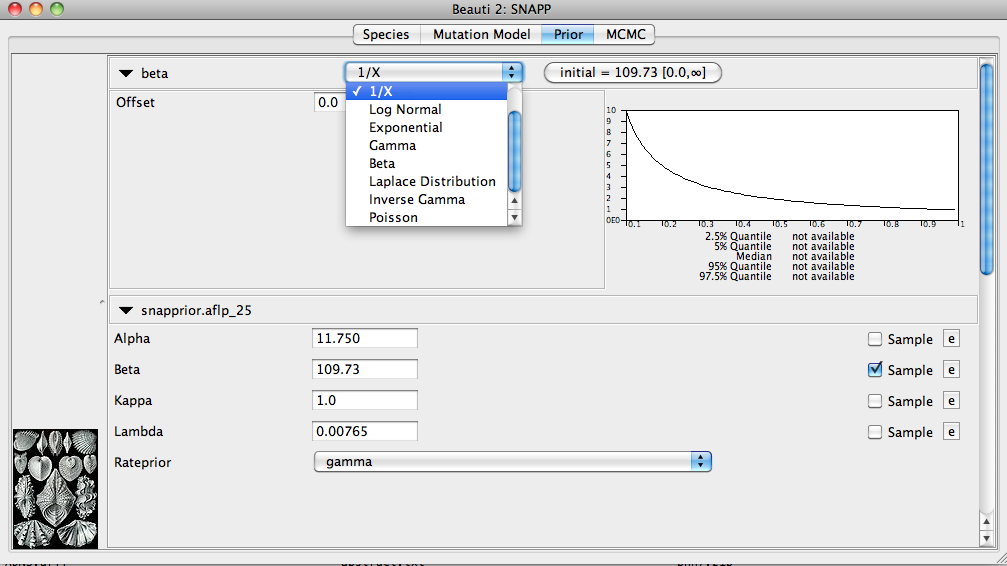
\includegraphics[width=0.75\textwidth]{figures/Beauti-prior2.png}
\end{center}
\end{minipage}


\subsubsection{Beauti MCMC settings}
Click the 'MCMC' tab to select parameters for the MCMC algorithm.
Under the log entries, file names and logging frequency can be specified 

\begin{minipage}{\textwidth}
\captionof{figure}{\label{fig.beauti6}MCMC settings in Beauti}
\begin{center}
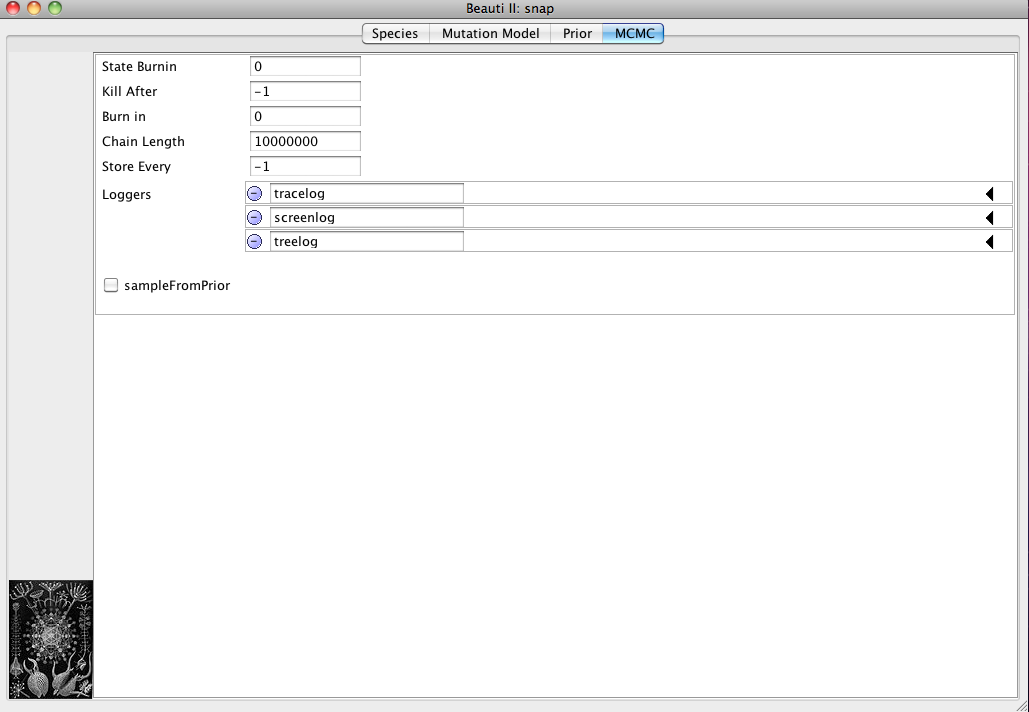
\includegraphics[width=0.75\textwidth]{figures/Beauti-mcmc.png}
\end{center}
\end{minipage}





\newpage
\newpage
\newpage

\section{Launching \SnAPhyl \label{sec.cmd}}

\SnAPhyl can be launched from the command line, or as a GUI application by double clicking the appropriate application.

When launching \SnAPhyl as GUI app, a window and dialog pop up as shown in Figure \ref{fig.launch}.

\begin{minipage}{\textwidth}
\captionof{figure}{\label{fig.launch}Launching \SnAPhyl}
\begin{center}
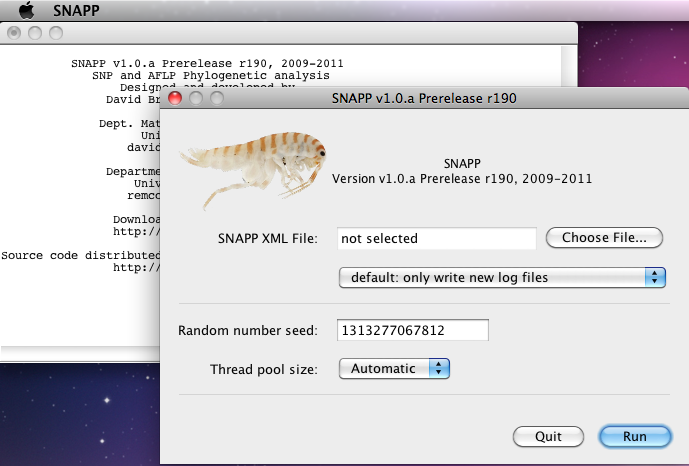
\includegraphics[width=0.75\textwidth]{figures/SNAPP.png}
\end{center}
\end{minipage}


\subsection{Command line options}

\begin{verbatim}
  Usage: snapp [-window] [-options] [-working] [-seed] [-prefix <PREFIX>] [-overwrite] [-resume] [-errors <i>] [-threads <i>] [-help] [<input-file-name>]
    -window Provide a console window
    -options Display an options dialog
    -working Change working directory to input file's directory
    -seed Specify a random number generator seed
    -prefix Specify a prefix for all output log filenames
    -overwrite Allow overwriting of log files
    -resume Allow appending of log files
    -errors Specify maximum number of numerical errors before stopping
    -threads The number of computational threads to use (default auto)
    -help Print this information and stop

  Example: snapp test.xml
  Example: snapp -window test.xml
  Example: snapp -help
\end{verbatim}

Some more detail on the options:

{\tt -seed} is the random number seed, which defaults to 667. Repeated runs with the same
seed result in the same outcomes. Running multiple chains with different seeds is recommended
to test for convergence.

{\tt -threads} specifies number of threads used. Increasing the number of threads will help on a
multi-core machine. Though the performance does not increase linearly with the number of thread, 
it does improves considerably, especially on many-core CPUs like the Intel i7.


\newpage
\section{Analyzing the Trace\label{sec.trace}}


Trace files generated by \SnAPhyl\ can be inspected using Tracer, which is part of BEAST.
Figure \ref{fig.trace} shows various screen shots of Tracer. The left hand (bottom) side shows mean
and effective sample size (ESS) for various variables. An ESS of less than 100 is generally an 
indication that the chain has not converged for that variable yet (expNumRootLineages in Figure 
\ref{fig.trace}). When ESS is larger than 100, the next thing to check is the shape of the trace.
If there are any obvious trends visible, or large fluctuations, this is generally a sign that the
chain has not converged. For example the middle plate of Figure \ref{fig.trace} shows the posterior
trace showing signs that it jumps between two states. However, if the chain converged, it should 
look closer to something like a hairy caterpillar shown at the bottom of Figure \ref{fig.trace}.

\begin{minipage}{\textwidth}
\captionof{figure}{\label{fig.trace}Various traces, from unacceptable to ok.}
\begin{center}
\includegraphics[width=0.48\textwidth]{figures/trace3.png}
\includegraphics[width=0.48\textwidth]{figures/trace2.png}
\includegraphics[width=1\textwidth]{figures/trace1.png}
\end{center}
%  \epsfig{width=110mm,file=trace3.eps}
%  \epsfig{width=110mm,file=trace2.eps}
%  \epsfig{width=110mm,file=trace1.eps}
\end{minipage}

\newpage
\section{Analyzing the Trees\label{sec.tree}}

\SnAPhyl\ can generate a tree set containing species trees.
There are various ways to analysing these tree sets.
\begin{itemize}
\item calculate a summary tree, e.g. through the tree annotator in BEAST.
The benefit is that a single tree is produced with 'error bars' on the position
of internal nodes. However, when there is a lot of uncertainty in the topology
of the species tree, this may not be directly obvious from the summary tree and
some skill is required to recognise these kind of situations.
\item calculate a set of clades with high frequency, e.g. through the tree log
analyser in BEAST. This will show a set of clades without the uncertainty in
node heights and the set can become quite large and hard to interpret.
\item Draw a consensus tree or consensus network (as in SplitsTree \cite{SplitsTree}), which is a graph 
containing edges wherever such edges appear (possibly at some threshold frequency)
in the tree set. 
\item Use multidimensional scaling (MDS) as for example implemented in 
\cite{treeviz2}. MDS allows identification
of tree islands in a compelling way, but uncertainty of node heights is hard
to interpret.
\item Draw a DensiTree \cite{DensiTree}, which shows the complete tree set
drawn transparently in a single image. Areas with hight uncertainty in the
tree topology will be easy to spot and distribtuion in node heights shows up
clearly as well.
\end{itemize}


{\tt TreeSetAnalyser} is a program that is part of the \SnAPhyl distribution. It reads in
a tree set file produced by \SnAPhyl and determines the distribution of topologies
of the species tree. Furthermore, it determines whether a pre-defined tree topology
(if any is specified) is in the 95\% HPD set of topologies. To start {\tt TreeSetAnalyser},
double click the TreeSetAnalyser icon and the following window should pop up.

\captionof{figure}{\label{fig.tsa}Tree set analyser}
\begin{center}
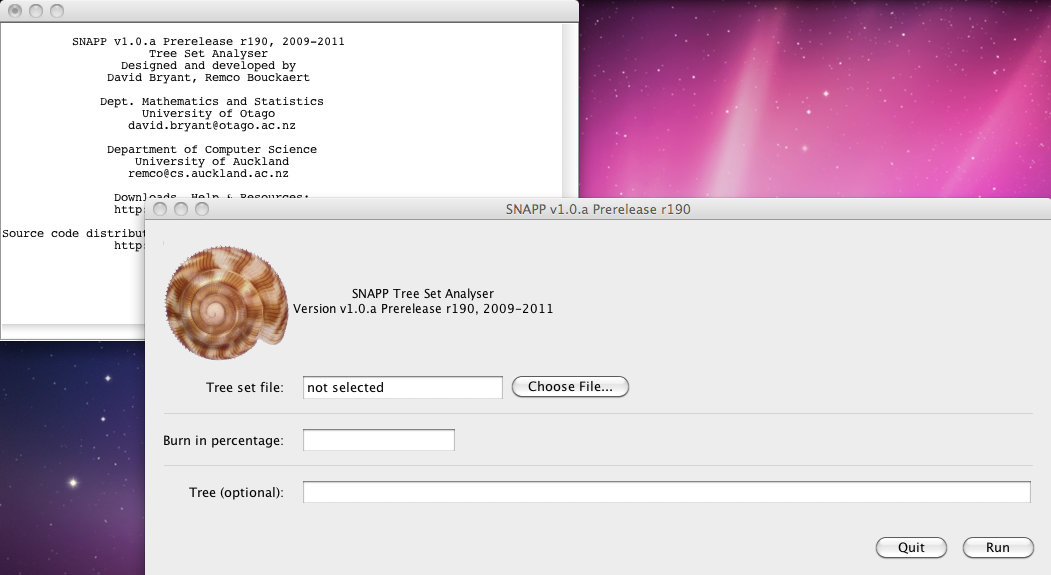
\includegraphics[width=0.8\textwidth]{figures/tsa.png}
\end{center}

By default, the burn in percentage is 10\%.
The Tree entry allows to specify a tree topology in Newick format.
When clicking Run, the results of the analysis are shows in the text window.

Figure \ref{fig.DensiTree} shows an example of a DensiTree.

\begin{minipage}{\textwidth}
\captionof{figure}{\label{fig.DensiTree}Example of a DensiTree. This highlights the uncertainty
in topology of the two 5-taxon clades. Also, note the increasing uncertainty in
internal node height going from the taxa to the root.}
\begin{center}

\includegraphics[width=0.8\textwidth]{figures/DensiTree.png}
\end{center}
\end{minipage}



One feature of {\tt DensiTreeS} is that it allows the branch thicknesses in a
tree to represent a parameter associated with a branch, such as $\theta$.
This figure can be exported as SVG file and manipulated in a drawing program
(e.g. PhotoShop, Gimp) to annotate a tree with extra information to produce
high quality ready for print images.


\newpage
\captionof{figure}{\label{fig.DensiTreeS}Example of a DensiTree showing only the 
dominating consensus tree where branch thickness represents $\theta$ associated
with the branch.}
\begin{center}

\includegraphics[width=0.8\textwidth]{figures/DensiTreeS.png}
\end{center}






\if0
\newpage
\section{File format\label{sec.format}}

\SnAPhyl\ uses the BEAST \cite{BEAST} file format, and in fact, can be processed 
by BEAST version XXXX or later. The difference between \SnAPhyl\ and BEAST is that
BEAST allows more operators, more MCMC options and possibly a richer set of models,
but this is at the cost of processing speed. Here, we describe the file format
which can be processed by both \SnAPhyl\ and BEAST.




\begin{verbatim}
<beast>
  <taxa id='taxa'>
    <taxon id='cae'>
            <attr name='totalcount'>15</attr>
    </taxon>
    <taxon id='cra'>
            <attr name='totalcount'>6</attr>
    </taxon>
    <taxon id='gla'>
            <attr name='totalcount'>6</attr>
    </taxon>
  </taxa>


  <alignment id='alignment' dataType='integerdata' statecount='16'>
    <sequence>
<taxon idref='cae'/>
0,1,1,0,0,1,1,...,13,14,14,14,15,15,15,15,15,15,15,15,</sequence>
    <sequence>
<taxon idref='cra'/>
0,0,0,0,0,0,0,...6,6,5,5,6,6,5,6,6,6,6,6,6,</sequence>
    <sequence>
<taxon idref='gla'/>
0,0,0,0,1,0,0,...,6,6,6,6,6,6,5,6,6,6,6,6,6,6,</sequence>
    <sequence>
  </alignment>
\end{verbatim}


Leave the pattern element (BEAST needs it). 
\begin{verbatim}
  <patterns id='patterns' from='1'>
         <alignment idref='alignment'/>
  </patterns>
\end{verbatim}

A block with parameters follows. These parameters contain the starting values 
(that is the values used at the start of the MCMC chain) for $u$, $v$, $\alpha$, $\beta$ 
and $\lambda$ respectively. When one wants to sample over these, a lower and upper
value can be provided, but they are not necessary when they remain constant over
the chain. For BEAST, it is required that the dimension attribute on the gamma
parameter is set to the number of internal nodes (= number of species times two minus one).
\begin{verbatim}
  <parameter id='u' value='3.33333' lower='0.0'/>
  <parameter id='v' value='0.588235' lower='0.0'/>
  <parameter id='alpha'  value='2.0' lower='0.0'/>
  <parameter id='beta'   value='12.0' lower='0.0'/>
  <parameter id='lambda' value='2.0' lower='0.0'/>
  <!-- dimension = #external nodes + #internal nodes = #taxa + #taxa-1 -->
  <parameter id='gamma' dimension="17" value='10.0'/>
\end{verbatim}

The starting tree (the tree used at the start of the MCMC chain) can be the UPGMA tree using the following element
\begin{verbatim}
  <upgmaTree id='startingTree'>
         <distanceMatrix correction='none'>
                 <patterns idref='patterns'/>
         </distanceMatrix>
  </upgmaTree>

\end{verbatim}

A starting tree can be specified using a string in Newick format.
\begin{verbatim}
  <newick id='startingTree'>
((0:0.000671398,2:0.000671398):0.000664729,1:0.00133613);
  </newick>
\end{verbatim}

If numbers in square brackets are provided, these are interpreted as $\theta$s ($\theta=2/\gamma$) for the nodes. 
If none are provided, the $\theta$ values will be generated from the prior.
\begin{verbatim}
  <newick id='startingTree'>
((0[0.00322648]:0.000671398,2[0.00271446]:0.000671398)[0.222576]:0.000664729,1[0.0132671]:0.00133613)[0.319135];
  </newick>
\end{verbatim}

If a completely random tree is required, the following fragment should be inserted in the XML.

\begin{verbatim}
  <constantSize id="initialDemo" units="substitutions">
         <populationSize>
                <parameter id="initialDemo.popSize" value="0.0001"/>
         </populationSize>
  </constantSize>
  <coalescentTree id='startingTree'>
        <taxa idref="taxa"/>
        <constantSize idref="initialDemo"/>
  </coalescentTree>

\end{verbatim}

The following fragment describes the relation between the components of the model, and should not be changed.

{\small
\begin{verbatim}
  <sssModel id='sss'>
         <alignment idref='alignment'/>
         <mutationRateV>
                 <parameter idref='v'/>
         </mutationRateV>
         <mutationRateU>
                 <parameter idref='u'/>
         </mutationRateU>
         <gamma>
                 <parameter idref='gamma'/>
         </gamma>
  </sssModel>

  <treeModel id='treeModel'>
         <tree idref='startingTree'/>
         <rootHeight>
                 <parameter id='treeModel.rootHeight'/>
         </rootHeight>
         <nodeHeights internalNodes='true'>
                 <parameter id='treeModel.internalNodeHeights'/>
         </nodeHeights>
         <nodeHeights internalNodes='true' rootNode='true'>
                 <parameter id='treeModel.allInternalNodeHeights'/>
         </nodeHeights>
  </treeModel>

  <sssTreeLikelihood id='treeLikelihood'>
        <patterns idref='patterns'/>
        <treeModel idref='treeModel'/>
        <sssModel idref='sss'/>

        <treeLength><parameter id="treeLength"/></treeLength>
        <treeHeight><parameter id="treeHeight"/></treeHeight>
        <expNumRootLineages><parameter id="expNumRootLineages"/></expNumRootLineages>
        <meanVarTheta><parameter id="meanVarTheta"/></meanVarTheta>
        <ThetaRoot><parameter id="ThetaRoot"/></ThetaRoot>
        <ESS><parameter id="ESS"/></ESS>
  </sssTreeLikelihood>
\end{verbatim}
}

The following block describes the operators used in the MCMC run. The weight attribute on the
operators determines the proportion of proposals with that particular operator. The following 
operators are available:
\begin{itemize}
\item nodeSwapper; randomly selects two leave nodes, randomly selects a time between leave and MRCA
and swaps subtrees at that point in time. Contains a treeModel attribute referring to the treeModel.
\item subtreeSlide; moves the height of a node in the interval between child and parent height.
The interval is multiplied by the value of the size attribute.
Contains a treeModel attribute referring to the treeModel.
\item scaleOperator; scales a parameter. When it contains a parameter referring to the rootHeight
of a tree, the height of the complete tree (including its nodes) are scaled.
\item gammaMove; selects a gamma value in a random node in the tree and scales it exponentially
$\gamma \leftarrow \gamma/e^{\kappa r}$ where $\kappa$ is the scale factor represented in
the pGammaMove attribute and $r$ a uniform random number between -1 and 1.
\item rateMixer; simultaneously scales all node heights and inverse-scales all gammas. The
scaleFactor attribute determines how much the size of the scaling is.
%\item mutationMover and  mutationScaler apply to mutation rates $u$ and $v$. 
%The mover changes the base frequencies without changing the average rate
% $v\leftarrow = v + \kappa r(u+v)$, $u \leftarrow u - \kappa r(u+v)$ where 
%$\kappa$ is the value of piWindow and $r$ a uniform random number between -1 and 1.
%The scaler changes them such that the condition $u+v=2uv$ is maintained. 
%The pMutationScaler attribute determines the size of the scaling.
%If it is required to sample over the mutation rate, the mutationMover and mutation
%the XML comment tags should be removed.
\end{itemize} 

{\small
\begin{verbatim}
    <operators id="operators">
        <nodeSwapper weight="0.5">
            <treeModel idref="treeModel"/>
        </nodeSwapper>
        <subtreeSlide weight="0.5" size="0.5">
            <treeModel idref="treeModel"/>
        </subtreeSlide>
        <scaleOperator scaleFactor="0.25" weight="0.5">
                <parameter idref="treeModel.rootHeight"/>
        </scaleOperator>
%<!--
%        <mutationmover piWindow="0.3" weight="0.00000000000000001">
%                <mutationRateU><parameter idref='u'/></mutationRateU>
%                <mutationRateV><parameter idref='v'/></mutationRateV>
%        </mutationmover>
%-->        
%<!--
%        <mutationscaler pMutationScaler="1.0" weight="0.00000000000000001">
%                <mutationRateU><parameter idref='u'/></mutationRateU>
%                <mutationRateV><parameter idref='v'/></mutationRateV>
%        </mutationscaler>
%-->        
        <gammaMover pGammaMove="0.5" weight="8">
                <parameter idref="gamma"/>
        </gammaMover>
        <ratemixer scaleFactors="0.25" weight="1">
                <mutationRateU><parameter idref='u'/></mutationRateU>
                <mutationRateV><parameter idref='v'/></mutationRateV>
        </ratemixer>
    </operators>
\end{verbatim}
}

The MCMC element has the following functions:
defining the length of the chain,
linking the elements of the posterior distribution and operators,
determining what is logged, where and when. 

The attributes chainLength determines the length of the chain, excluding preBurnin.
The preBurning attribute (default 0) determines the number of samples generated
before the start of the chain, that are completely ignored.

The posterior element contains references to the prior and likelihood, and should not
be changed. Likewise, the operators element contains a reference to the operators
described above and should not be changed.

\begin{verbatim}
    <mcmc id="mcmc" chainLength="10000000" preBurnin="0" autoOptimize="true">
        <posterior id="posterior">
            <prior id="prior">
                <sssPrior lowerGamma="0.0">
                        <alpha> <parameter idref='alpha'/> </alpha>
                        <beta>  <parameter idref='beta'/> </beta>
                        <lambda><parameter idref='lambda'/> </lambda>
                        <mutationRateU><parameter idref='u'/></mutationRateU>
                        <mutationRateV><parameter idref='v'/></mutationRateV>
                        <gamma><parameter idref='gamma'/></gamma>
                        <treeModel idref='treeModel'/>
                </sssPrior>
            </prior>
            <likelihood id='likelihood'>
                <treeLikelihood idref="treeLikelihood"/>
            </likelihood>
        </posterior>
        <operators idref="operators"/>
\end{verbatim}


Logging can be done on screen and to a file. It produces logs that can be processes by
the tracer application. The logEvery attribute determines how many samples are skipped 
before the sample is shown. The filename attribute is optional. If not provided, the
logger reports to standard output. Otherwise, it writes the log in a file. If the attribute
contains {\tt\$(seed)} this will be replaced by the seed used to run the chain in \SnAPhyl
though it will be ignored in BEAST.

The column elements have no effect in \SnAPhyl\ but help formatting in BEAST.

The following items can be reported; prior, likelihood, posterior. The values of any
of the parameters. Some special build in functions, namely treeLength (sum of length
of branches in tree), treeHeight (height of the root), 
treeLengthG (as treeLength, but multiplied by the gamma for each node), 
treeHeightG (as treeHeight, but multiplied by the gamma for each node), 
expNumRootLineages (expected number of root lineages), 
meanVarTheta (mean and variance of $\theta$) and 
ThetaRoot ($\theta$ of the root node).

\begin{verbatim}
        <log logEvery="1">
            <parameter idref="u"/>
            <parameter idref="v"/>
            <column label="Prior" sf="6" width="12">
                    <prior idref="prior"/>
            </column>
            <column label="Likelihood" dp="4" width="12">
                    <likelihood idref="likelihood"/>
            </column>
            <column label="Posterior" dp="4" width="12">
                <posterior idref="posterior"/>
            </column>

            <column label="meanVarTheta" sf="6" width="12">
                    <parameter idref="meanVarTheta"/>
            </column>
            <column label="ThetaRoot" sf="6" width="12">
                    <parameter idref="ThetaRoot"/>
            </column>
            <parameter idref="treeLengthG"/>
            <parameter idref="treeHeightG"/>
        </log>
        <log logEvery="100" fileName="test.$(seed).log">
            <prior idref="prior"/>
            <likelihood idref="likelihood"/>
            <posterior idref="posterior"/>
            <parameter idref="u"/>
            <parameter idref="v"/>
            <parameter idref="treeLength"/>
            <parameter idref="treeHeight"/>
            <parameter idref="treeLengthG"/>
            <parameter idref="treeHeightG"/>
            <parameter idref="expNumRootLineages"/>
            <parameter idref="meanVarTheta"/>
            <parameter idref="ThetaRoot"/>
        </log>
\end{verbatim}

To log trees in nexus format so that e.g. figtree can read them, the logTree element should be used and 
it has a logEvery and fileName attribute that behave like the log element. 

\begin{verbatim}
        <logTree logEvery="100" nexusFormat="true" fileName="test.$(seed).trees">
            <treeModel idref="treeModel"/>
        </logTree>
    </mcmc>
</beast>
\end{verbatim}
\fi 

\newpage
\bibliographystyle{plain}
\begin{thebibliography}{1}
\bibitem{BEAST}
        A Drummond and A Rambaut. BEAST: Bayesian evolutionary analysis by sampling trees.
        BMC Evolutionary Biology, Jan 2007.
\bibitem{SnAPhyl} 
	David Bryant, Remco Bouckaert, Joseph Felsenstein, Noah Rosenberg, Arindam RoyChoudhury. 
	Inferring Species Trees Directly from Biallelic Genetic Markers: Bypassing Gene Trees in a Full Coalescent Analysis. 
	Mol. Biol. Evol. 29(8):1917-1932, 2012
\bibitem{SplitsTree}
	D. H. Huson and D. Bryant. 
	Application of Phylogenetic Networks in Evolutionary Studies, Mol. Biol. Evol., 23(2):254-267, 2006.
	\url{http://www.splitstree.org/}
\bibitem{DensiTree}
	Remco R. Bouckaert.
	DensiTree: making sense of sets of phylogenetic trees
	Bioinformatics, Vol. 26, No. 10. (15 May 2010), pp. 1372-1373.
\bibitem{treeviz2}
	Hillis, D.M., Heath, T.A. and St John, K.
	Analysis and Visualization of Tree Space. 
	Syst. Biol. 54(3):471-82, 2005.
\bibitem{CIR}
    Cox, J.C., J.E. Ingersoll and S.A. Ross. "A Theory of the Term Structure of Interest Rates". Econometrica 53: 385–407, 1985.
%\bibitem{Tanjya}Paper on Yule prior???
\end{thebibliography}

\end{document}

